\documentclass{book}
\usepackage[a4paper,top=2.5cm,bottom=2.5cm,left=2.5cm,right=2.5cm]{geometry}
\usepackage{makeidx}
\usepackage{natbib}
\usepackage{graphicx}
\usepackage{multicol}
\usepackage{float}
\usepackage{listings}
\usepackage{color}
\usepackage{ifthen}
\usepackage[table]{xcolor}
\usepackage{textcomp}
\usepackage{alltt}
\usepackage{ifpdf}
\ifpdf
\usepackage[pdftex,
            pagebackref=true,
            colorlinks=true,
            linkcolor=blue,
            unicode
           ]{hyperref}
\else
\usepackage[ps2pdf,
            pagebackref=true,
            colorlinks=true,
            linkcolor=blue,
            unicode
           ]{hyperref}
\usepackage{pspicture}
\fi
\usepackage[utf8]{inputenc}
\usepackage{mathptmx}
\usepackage[scaled=.90]{helvet}
\usepackage{courier}
\usepackage{sectsty}
\usepackage{amssymb}
\usepackage[titles]{tocloft}
\usepackage{doxygen}
\lstset{language=C++,inputencoding=utf8,basicstyle=\footnotesize,breaklines=true,breakatwhitespace=true,tabsize=4,numbers=left }
\makeindex
\setcounter{tocdepth}{3}
\renewcommand{\footrulewidth}{0.4pt}
\renewcommand{\familydefault}{\sfdefault}
\hfuzz=15pt
\setlength{\emergencystretch}{15pt}
\hbadness=750
\tolerance=750
\begin{document}
\hypersetup{pageanchor=false,citecolor=blue}
\begin{titlepage}
\vspace*{7cm}
\begin{center}
{\Large Uikun }\\
\vspace*{1cm}
{\large Generated by Doxygen 1.8.3.1}\\
\vspace*{0.5cm}
{\small Tue Jul 23 2013 19:49:14}\\
\end{center}
\end{titlepage}
\clearemptydoublepage
\pagenumbering{roman}
\tableofcontents
\clearemptydoublepage
\pagenumbering{arabic}
\hypersetup{pageanchor=true,citecolor=blue}
\chapter{Hierarchical Index}
\section{Class Hierarchy}
This inheritance list is sorted roughly, but not completely, alphabetically\-:\begin{DoxyCompactList}
\item \contentsline{section}{Arc\-Ball\-\_\-t}{\pageref{classArcBall__t}}{}
\item \contentsline{section}{pho\-:\-:Box}{\pageref{classpho_1_1Box}}{}
\item \contentsline{section}{pho\-:\-:Buttons}{\pageref{structpho_1_1Buttons}}{}
\item \contentsline{section}{pho\-:\-:Event\-Queue}{\pageref{classpho_1_1EventQueue}}{}
\item \contentsline{section}{pho\-:\-:flick\-Manager}{\pageref{classpho_1_1flickManager}}{}
\item \contentsline{section}{Minicom\-\_\-client}{\pageref{classMinicom__client}}{}
\item Tuio\-Listener\begin{DoxyCompactList}
\item \contentsline{section}{pho\-:\-:Engine}{\pageref{classpho_1_1Engine}}{}
\item \contentsline{section}{pho\-:\-:My\-Tuio\-Listener}{\pageref{classpho_1_1MyTuioListener}}{}
\end{DoxyCompactList}
\item \contentsline{section}{udp\-\_\-server}{\pageref{classudp__server}}{}
\item \contentsline{section}{pho\-:\-:Vector3}{\pageref{classpho_1_1Vector3}}{}
\item \contentsline{section}{pho\-:\-:Wii\-Button\-State}{\pageref{classpho_1_1WiiButtonState}}{}
\end{DoxyCompactList}

\chapter{Class Index}
\section{Class List}
Here are the classes, structs, unions and interfaces with brief descriptions\-:\begin{DoxyCompactList}
\item\contentsline{section}{\hyperlink{classArcBall__t}{Arc\-Ball\-\_\-t} }{\pageref{classArcBall__t}}{}
\item\contentsline{section}{\hyperlink{classpho_1_1Box}{pho\-::\-Box} }{\pageref{classpho_1_1Box}}{}
\item\contentsline{section}{\hyperlink{structpho_1_1Buttons}{pho\-::\-Buttons} }{\pageref{structpho_1_1Buttons}}{}
\item\contentsline{section}{\hyperlink{classpho_1_1Engine}{pho\-::\-Engine} }{\pageref{classpho_1_1Engine}}{}
\item\contentsline{section}{\hyperlink{classpho_1_1EventQueue}{pho\-::\-Event\-Queue} }{\pageref{classpho_1_1EventQueue}}{}
\item\contentsline{section}{\hyperlink{classpho_1_1flickManager}{pho\-::flick\-Manager} }{\pageref{classpho_1_1flickManager}}{}
\item\contentsline{section}{\hyperlink{classMinicom__client}{Minicom\-\_\-client} }{\pageref{classMinicom__client}}{}
\item\contentsline{section}{\hyperlink{classpho_1_1MyTuioListener}{pho\-::\-My\-Tuio\-Listener} }{\pageref{classpho_1_1MyTuioListener}}{}
\item\contentsline{section}{\hyperlink{classudp__server}{udp\-\_\-server} }{\pageref{classudp__server}}{}
\item\contentsline{section}{\hyperlink{classpho_1_1Vector3}{pho\-::\-Vector3} }{\pageref{classpho_1_1Vector3}}{}
\item\contentsline{section}{\hyperlink{classpho_1_1WiiButtonState}{pho\-::\-Wii\-Button\-State} }{\pageref{classpho_1_1WiiButtonState}}{}
\end{DoxyCompactList}

\chapter{Class Documentation}
\hypertarget{classArcBall__t}{\section{Arc\-Ball\-\_\-t Class Reference}
\label{classArcBall__t}\index{Arc\-Ball\-\_\-t@{Arc\-Ball\-\_\-t}}
}
\subsection*{Public Member Functions}
\begin{DoxyCompactItemize}
\item 
\hypertarget{classArcBall__t_af0ab0bc3512889d777ad49dd7dfe388d}{{\bfseries Arc\-Ball\-\_\-t} (G\-Lfloat New\-Width, G\-Lfloat New\-Height)}\label{classArcBall__t_af0ab0bc3512889d777ad49dd7dfe388d}

\item 
\hypertarget{classArcBall__t_acc0216248bfd6d0b390c667a717fe881}{void {\bfseries set\-Bounds} (G\-Lfloat New\-Width, G\-Lfloat New\-Height)}\label{classArcBall__t_acc0216248bfd6d0b390c667a717fe881}

\item 
\hypertarget{classArcBall__t_ab457e36f9ef611c43d811e08c0100a74}{void {\bfseries click} (const vec2 $\ast$New\-Pt)}\label{classArcBall__t_ab457e36f9ef611c43d811e08c0100a74}

\item 
\hypertarget{classArcBall__t_a9902ea6c869db89bdadc393c362dd526}{void {\bfseries drag} (const vec2 $\ast$New\-Pt, quat $\ast$New\-Rot)}\label{classArcBall__t_a9902ea6c869db89bdadc393c362dd526}

\end{DoxyCompactItemize}
\subsection*{Protected Member Functions}
\begin{DoxyCompactItemize}
\item 
\hypertarget{classArcBall__t_a23147b991684651894ae66e89452d23d}{void {\bfseries \-\_\-map\-To\-Sphere} (const vec2 $\ast$New\-Pt, vec3 $\ast$New\-Vec) const }\label{classArcBall__t_a23147b991684651894ae66e89452d23d}

\end{DoxyCompactItemize}
\subsection*{Protected Attributes}
\begin{DoxyCompactItemize}
\item 
\hypertarget{classArcBall__t_a1ea7817b9e59153dd13d8c776ad1ec82}{vec3 {\bfseries St\-Vec}}\label{classArcBall__t_a1ea7817b9e59153dd13d8c776ad1ec82}

\item 
\hypertarget{classArcBall__t_abbbe14879d015fa4d2bf396b25ba5f2a}{vec3 {\bfseries En\-Vec}}\label{classArcBall__t_abbbe14879d015fa4d2bf396b25ba5f2a}

\item 
\hypertarget{classArcBall__t_a138f84b43a9fe26efb46734c93b782a0}{G\-Lfloat {\bfseries Adjust\-Width}}\label{classArcBall__t_a138f84b43a9fe26efb46734c93b782a0}

\item 
\hypertarget{classArcBall__t_ae5f8b2ea648b41ee1952dcdcd3857059}{G\-Lfloat {\bfseries Adjust\-Height}}\label{classArcBall__t_ae5f8b2ea648b41ee1952dcdcd3857059}

\end{DoxyCompactItemize}


The documentation for this class was generated from the following files\-:\begin{DoxyCompactItemize}
\item 
arcball.\-h\item 
arcball.\-cpp\end{DoxyCompactItemize}

\hypertarget{classpho_1_1Box}{\section{pho\-:\-:Box Class Reference}
\label{classpho_1_1Box}\index{pho\-::\-Box@{pho\-::\-Box}}
}
\subsection*{Public Member Functions}
\begin{DoxyCompactItemize}
\item 
\hypertarget{classpho_1_1Box_a08032b3766c61526c555651c434d5bec}{{\bfseries Box} (const \hyperlink{classpho_1_1Vector3}{Vector3} \&min, const \hyperlink{classpho_1_1Vector3}{Vector3} \&max)}\label{classpho_1_1Box_a08032b3766c61526c555651c434d5bec}

\item 
\hypertarget{classpho_1_1Box_a2ebbc99e20bf99038d07856b2d05fbed}{bool {\bfseries intersect} (const Ray \&, float t0, float t1) const }\label{classpho_1_1Box_a2ebbc99e20bf99038d07856b2d05fbed}

\end{DoxyCompactItemize}
\subsection*{Public Attributes}
\begin{DoxyCompactItemize}
\item 
\hypertarget{classpho_1_1Box_ac74266938b9d2c47be56c4ec553c7e8e}{\hyperlink{classpho_1_1Vector3}{Vector3} {\bfseries parameters} \mbox{[}2\mbox{]}}\label{classpho_1_1Box_ac74266938b9d2c47be56c4ec553c7e8e}

\end{DoxyCompactItemize}


The documentation for this class was generated from the following files\-:\begin{DoxyCompactItemize}
\item 
box.\-h\item 
box.\-cc\end{DoxyCompactItemize}

\hypertarget{structpho_1_1Buttons}{\section{pho\-:\-:Buttons Struct Reference}
\label{structpho_1_1Buttons}\index{pho\-::\-Buttons@{pho\-::\-Buttons}}
}
\subsection*{Public Attributes}
\begin{DoxyCompactItemize}
\item 
\hypertarget{structpho_1_1Buttons_ad98663dc38ea19e05acb20cb1726fac4}{\hyperlink{classpho_1_1WiiButtonState}{Wii\-Button\-State} {\bfseries wiimote}}\label{structpho_1_1Buttons_ad98663dc38ea19e05acb20cb1726fac4}

\item 
\hypertarget{structpho_1_1Buttons_a680e4b82f639fc59cb0ee9a751a98671}{bool {\bfseries mouse1}}\label{structpho_1_1Buttons_a680e4b82f639fc59cb0ee9a751a98671}

\item 
\hypertarget{structpho_1_1Buttons_a533d8810438659b329ad87e044a74edb}{bool {\bfseries mouse2}}\label{structpho_1_1Buttons_a533d8810438659b329ad87e044a74edb}

\item 
\hypertarget{structpho_1_1Buttons_a31c8503c8087311a0b91133fd9c95cb8}{bool {\bfseries sn\-Button1}}\label{structpho_1_1Buttons_a31c8503c8087311a0b91133fd9c95cb8}

\item 
\hypertarget{structpho_1_1Buttons_a02a2249c571a454f53a908735a22d66a}{bool {\bfseries sn\-Button2}}\label{structpho_1_1Buttons_a02a2249c571a454f53a908735a22d66a}

\item 
\hypertarget{structpho_1_1Buttons_a208cc9a8d960e7b3a3f3e6854a1cf909}{bool {\bfseries phone\-Volume\-Up}}\label{structpho_1_1Buttons_a208cc9a8d960e7b3a3f3e6854a1cf909}

\item 
\hypertarget{structpho_1_1Buttons_ab403d4cd5169702a714bb2f2d479ff74}{bool {\bfseries phone\-Volume\-Down}}\label{structpho_1_1Buttons_ab403d4cd5169702a714bb2f2d479ff74}

\item 
\hypertarget{structpho_1_1Buttons_ac506deb5bf06d3a7480eda5f9317b406}{bool {\bfseries phone\-Button\-Touch}}\label{structpho_1_1Buttons_ac506deb5bf06d3a7480eda5f9317b406}

\end{DoxyCompactItemize}


The documentation for this struct was generated from the following file\-:\begin{DoxyCompactItemize}
\item 
util.\-h\end{DoxyCompactItemize}

\hypertarget{classpho_1_1Engine}{\section{pho\-:\-:Engine Class Reference}
\label{classpho_1_1Engine}\index{pho\-::\-Engine@{pho\-::\-Engine}}
}
Inheritance diagram for pho\-:\-:Engine\-:\begin{figure}[H]
\begin{center}
\leavevmode
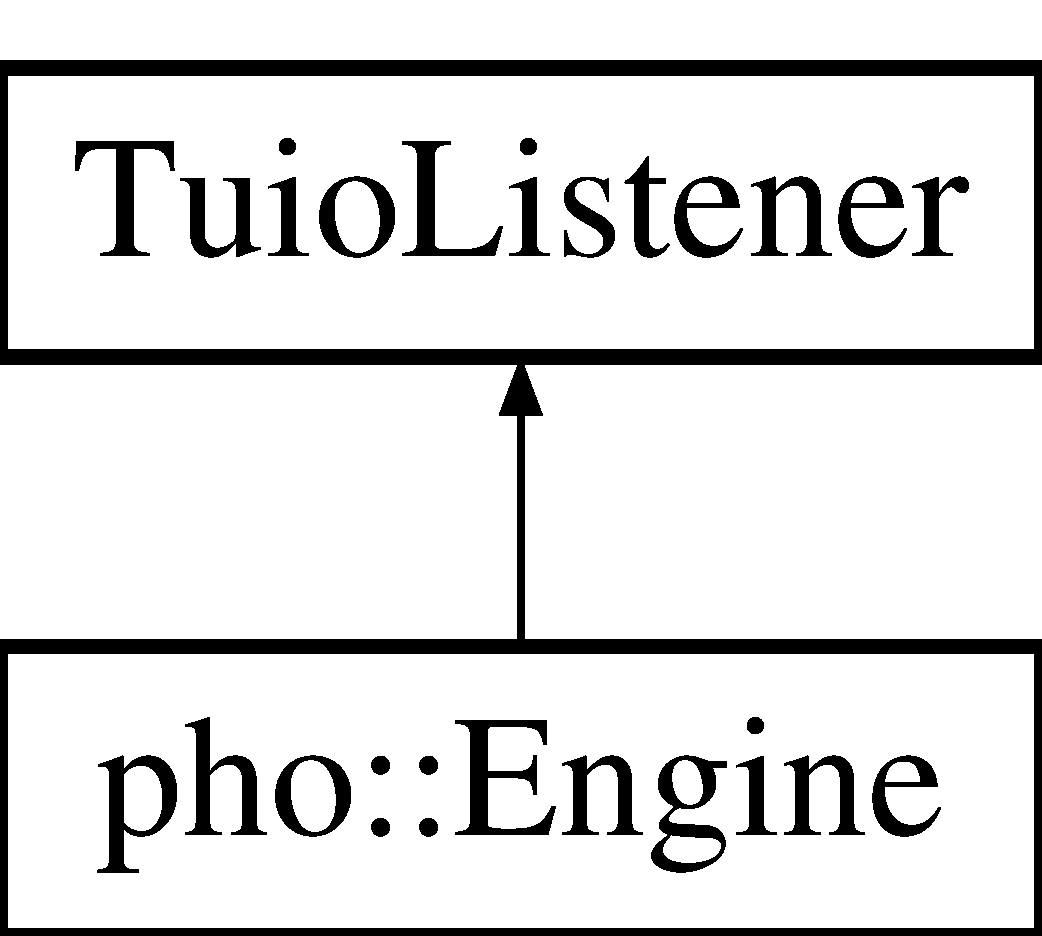
\includegraphics[height=2.000000cm]{classpho_1_1Engine}
\end{center}
\end{figure}
\subsection*{Public Member Functions}
\begin{DoxyCompactItemize}
\item 
\hypertarget{classpho_1_1Engine_a815f596ba518b16632f2e47e8921bf71}{void {\bfseries check\-Events} ()}\label{classpho_1_1Engine_a815f596ba518b16632f2e47e8921bf71}

\item 
\hypertarget{classpho_1_1Engine_a7960743aefd62e846e7f3cd92c18bc73}{void {\bfseries render} ()}\label{classpho_1_1Engine_a7960743aefd62e846e7f3cd92c18bc73}

\item 
\hypertarget{classpho_1_1Engine_ad2fa8d8efa0a9877f5aba94137b8b374}{void {\bfseries recursive\-\_\-render} (const struct ai\-Scene $\ast$sc, const struct ai\-Node $\ast$nd)}\label{classpho_1_1Engine_ad2fa8d8efa0a9877f5aba94137b8b374}

\item 
\hypertarget{classpho_1_1Engine_a4437ae8ba19d5c9800e0155cae37cae7}{void {\bfseries init\-Resources} ()}\label{classpho_1_1Engine_a4437ae8ba19d5c9800e0155cae37cae7}

\item 
\hypertarget{classpho_1_1Engine_a8b35e79b79a49b1e344681183d73bc5b}{void {\bfseries go} ()}\label{classpho_1_1Engine_a8b35e79b79a49b1e344681183d73bc5b}

\item 
\hypertarget{classpho_1_1Engine_a392c7c42460184c3993046a2c877e443}{bool {\bfseries compute\-Rotation\-Matrix} ()}\label{classpho_1_1Engine_a392c7c42460184c3993046a2c877e443}

\item 
\hypertarget{classpho_1_1Engine_a4bbccf668c46064559c99a999f7b9932}{void {\bfseries shutdown} ()}\label{classpho_1_1Engine_a4bbccf668c46064559c99a999f7b9932}

\item 
\hypertarget{classpho_1_1Engine_a2fe85c12b0537175ff02abd425dbaec9}{void {\bfseries mouse\-Button\-Callback} (int x, int y)}\label{classpho_1_1Engine_a2fe85c12b0537175ff02abd425dbaec9}

\item 
\hypertarget{classpho_1_1Engine_aacd64b3ed97712d730fdb660632a49e4}{void {\bfseries mouse\-Move\-Callback} (int x, int y)}\label{classpho_1_1Engine_aacd64b3ed97712d730fdb660632a49e4}

\item 
\hypertarget{classpho_1_1Engine_a226682d9f6f087a5808e6eb21b330b01}{void {\bfseries add\-Tuio\-Object} (Tuio\-Object $\ast$tobj)}\label{classpho_1_1Engine_a226682d9f6f087a5808e6eb21b330b01}

\item 
\hypertarget{classpho_1_1Engine_ae08af0370a3277418f1cbad6f293995f}{void {\bfseries update\-Tuio\-Object} (Tuio\-Object $\ast$tobj)}\label{classpho_1_1Engine_ae08af0370a3277418f1cbad6f293995f}

\item 
\hypertarget{classpho_1_1Engine_ab64f95319532116ab75afd4140ab0af8}{void {\bfseries remove\-Tuio\-Object} (Tuio\-Object $\ast$tobj)}\label{classpho_1_1Engine_ab64f95319532116ab75afd4140ab0af8}

\item 
\hypertarget{classpho_1_1Engine_a0e50e8111b9a2da5a4f46bd716d049b2}{void {\bfseries add\-Tuio\-Cursor} (Tuio\-Cursor $\ast$tcur)}\label{classpho_1_1Engine_a0e50e8111b9a2da5a4f46bd716d049b2}

\item 
\hypertarget{classpho_1_1Engine_ad3c836022d6b6ddc37cb1c0e5d6eb376}{void {\bfseries update\-Tuio\-Cursor} (Tuio\-Cursor $\ast$tcur)}\label{classpho_1_1Engine_ad3c836022d6b6ddc37cb1c0e5d6eb376}

\item 
\hypertarget{classpho_1_1Engine_a7135ab4aa02dd55685c144d1291cd7bf}{void {\bfseries remove\-Tuio\-Cursor} (Tuio\-Cursor $\ast$tcur)}\label{classpho_1_1Engine_a7135ab4aa02dd55685c144d1291cd7bf}

\end{DoxyCompactItemize}
\subsection*{Public Attributes}
\begin{DoxyCompactItemize}
\item 
\hypertarget{classpho_1_1Engine_a3cc0d353df3842afa2aca086c4237b97}{Tuio\-Client $\ast$ {\bfseries tuio\-Client}}\label{classpho_1_1Engine_a3cc0d353df3842afa2aca086c4237b97}

\end{DoxyCompactItemize}
\subsection*{Static Public Attributes}
\begin{DoxyCompactItemize}
\item 
\hypertarget{classpho_1_1Engine_af6adbe230aed4052bfc7933e34779a45}{static const int {\bfseries T\-O\-U\-C\-H\-\_\-\-S\-C\-R\-E\-E\-N\-\_\-\-S\-I\-Z\-E\-\_\-\-X} = 480}\label{classpho_1_1Engine_af6adbe230aed4052bfc7933e34779a45}

\item 
\hypertarget{classpho_1_1Engine_aabf7a0400411c35a5fcf3f0a7e48eeb2}{static const int {\bfseries T\-O\-U\-C\-H\-\_\-\-S\-C\-R\-E\-E\-N\-\_\-\-S\-I\-Z\-E\-\_\-\-Y} = 800}\label{classpho_1_1Engine_aabf7a0400411c35a5fcf3f0a7e48eeb2}

\item 
\hypertarget{classpho_1_1Engine_a4e1b0277c05451700ad1e0d7b76b22eb}{static const int {\bfseries W\-I\-N\-D\-O\-W\-\_\-\-S\-I\-Z\-E\-\_\-\-X} = 800}\label{classpho_1_1Engine_a4e1b0277c05451700ad1e0d7b76b22eb}

\item 
\hypertarget{classpho_1_1Engine_a25016d27a909cd81e3d0706c36f2489c}{static const int {\bfseries W\-I\-N\-D\-O\-W\-\_\-\-S\-I\-Z\-E\-\_\-\-Y} = 600}\label{classpho_1_1Engine_a25016d27a909cd81e3d0706c36f2489c}

\end{DoxyCompactItemize}


The documentation for this class was generated from the following files\-:\begin{DoxyCompactItemize}
\item 
uikun.\-h\item 
uikun.\-cpp\end{DoxyCompactItemize}

\hypertarget{classpho_1_1EventQueue}{\section{pho\-:\-:Event\-Queue Class Reference}
\label{classpho_1_1EventQueue}\index{pho\-::\-Event\-Queue@{pho\-::\-Event\-Queue}}
}
\subsection*{Public Member Functions}
\begin{DoxyCompactItemize}
\item 
\hypertarget{classpho_1_1EventQueue_a8c35e3bd373ab5df1cdc091a3ab5439f}{void {\bfseries push} (keimote\-::\-Phone\-Event event)}\label{classpho_1_1EventQueue_a8c35e3bd373ab5df1cdc091a3ab5439f}

\item 
\hypertarget{classpho_1_1EventQueue_a4ce35212696d3ae18e2ac6801733d6ca}{void {\bfseries push} (boost\-::array$<$ float, 7 $>$)}\label{classpho_1_1EventQueue_a4ce35212696d3ae18e2ac6801733d6ca}

\item 
\hypertarget{classpho_1_1EventQueue_a640119cdaa3573d8ed0f7664faae6ec4}{bool {\bfseries is\-Empty} ()}\label{classpho_1_1EventQueue_a640119cdaa3573d8ed0f7664faae6ec4}

\item 
\hypertarget{classpho_1_1EventQueue_af652b05c591ba0a166a9a60847f9cb7d}{bool {\bfseries is\-Serial\-Empty} ()}\label{classpho_1_1EventQueue_af652b05c591ba0a166a9a60847f9cb7d}

\item 
\hypertarget{classpho_1_1EventQueue_ac20b80f15fc7e02b809487213fe76cc1}{keimote\-::\-Phone\-Event {\bfseries pop} ()}\label{classpho_1_1EventQueue_ac20b80f15fc7e02b809487213fe76cc1}

\item 
\hypertarget{classpho_1_1EventQueue_ac6d27beddc1129d8f42204d0fe00d4ce}{boost\-::array$<$ float, 7 $>$ {\bfseries serial\-Pop} ()}\label{classpho_1_1EventQueue_ac6d27beddc1129d8f42204d0fe00d4ce}

\item 
\hypertarget{classpho_1_1EventQueue_aedbec8b87281f1c2b070df9d92faf917}{void {\bfseries set\-Technique} (Input\-Technique new\-Technique)}\label{classpho_1_1EventQueue_aedbec8b87281f1c2b070df9d92faf917}

\item 
\hypertarget{classpho_1_1EventQueue_ae03b167d6ac48dd2b45fce2a46d228d6}{void {\bfseries set\-App} (App new\-App)}\label{classpho_1_1EventQueue_ae03b167d6ac48dd2b45fce2a46d228d6}

\item 
\hypertarget{classpho_1_1EventQueue_a8b0dac3ce56de908914461d93716c33d}{Input\-Technique {\bfseries get\-Technique} ()}\label{classpho_1_1EventQueue_a8b0dac3ce56de908914461d93716c33d}

\item 
\hypertarget{classpho_1_1EventQueue_a3b9d803d2ac2f0514da964852bcd5ba8}{App {\bfseries get\-App} ()}\label{classpho_1_1EventQueue_a3b9d803d2ac2f0514da964852bcd5ba8}

\end{DoxyCompactItemize}


The documentation for this class was generated from the following files\-:\begin{DoxyCompactItemize}
\item 
event\-Queue.\-h\item 
event\-Queue.\-cpp\end{DoxyCompactItemize}

\hypertarget{classpho_1_1flickManager}{\section{pho\-:\-:flick\-Manager Class Reference}
\label{classpho_1_1flickManager}\index{pho\-::flick\-Manager@{pho\-::flick\-Manager}}
}
\subsection*{Public Member Functions}
\begin{DoxyCompactItemize}
\item 
\hypertarget{classpho_1_1flickManager_ad9f5cb98e758564c5ebc913d9aa120d1}{void {\bfseries add\-Touch} (glm\-::vec2 speeds)}\label{classpho_1_1flickManager_ad9f5cb98e758564c5ebc913d9aa120d1}

\item 
\hypertarget{classpho_1_1flickManager_a1b1df3626e566e118b936ad3e4005243}{void {\bfseries add\-Rotate} (float angle)}\label{classpho_1_1flickManager_a1b1df3626e566e118b936ad3e4005243}

\item 
\hypertarget{classpho_1_1flickManager_a653c945f19ae5a056851aa3a9ab1f805}{void {\bfseries end\-Flick} (glm\-::mat3 orientation\-Snapshot)}\label{classpho_1_1flickManager_a653c945f19ae5a056851aa3a9ab1f805}

\item 
\hypertarget{classpho_1_1flickManager_a46786fd5133be5792a9e9ffd2ba912e6}{void {\bfseries end\-Pinch\-Flick} ()}\label{classpho_1_1flickManager_a46786fd5133be5792a9e9ffd2ba912e6}

\item 
\hypertarget{classpho_1_1flickManager_abe57e168a8cf3a3f7953339fd75e143b}{void {\bfseries end\-Rotation\-Flick} ()}\label{classpho_1_1flickManager_abe57e168a8cf3a3f7953339fd75e143b}

\item 
\hypertarget{classpho_1_1flickManager_acdb07c082db311651ff014c04540abcf}{void {\bfseries stop\-Flick} ()}\label{classpho_1_1flickManager_acdb07c082db311651ff014c04540abcf}

\item 
\hypertarget{classpho_1_1flickManager_a12979db47dee255a954a8ba07e1da436}{void {\bfseries stop\-Pinch\-Flick} ()}\label{classpho_1_1flickManager_a12979db47dee255a954a8ba07e1da436}

\item 
\hypertarget{classpho_1_1flickManager_a32ec82aea2ccc84487233d25ff0c1b30}{glm\-::mat4 {\bfseries dampen\-And\-Give\-Matrix} (glm\-::mat3 rotation\-Mat)}\label{classpho_1_1flickManager_a32ec82aea2ccc84487233d25ff0c1b30}

\item 
\hypertarget{classpho_1_1flickManager_a413def44a7b636a274657ceb51d67baa}{glm\-::mat4 {\bfseries dampen\-And\-Give\-Pinch\-Matrix} ()}\label{classpho_1_1flickManager_a413def44a7b636a274657ceb51d67baa}

\item 
\hypertarget{classpho_1_1flickManager_af442fac3135f7e5bec29197c995b54d4}{glm\-::vec2 {\bfseries dampen\-And\-Give\-Rotation\-Matrix} ()}\label{classpho_1_1flickManager_af442fac3135f7e5bec29197c995b54d4}

\item 
\hypertarget{classpho_1_1flickManager_aec9a8e9bb6327725b8695a8fc9e4db33}{void {\bfseries new\-Flick} ()}\label{classpho_1_1flickManager_aec9a8e9bb6327725b8695a8fc9e4db33}

\item 
\hypertarget{classpho_1_1flickManager_a598ab994f75f782dd469c4f0c460b6d2}{bool {\bfseries in\-Flick} ()}\label{classpho_1_1flickManager_a598ab994f75f782dd469c4f0c460b6d2}

\item 
\hypertarget{classpho_1_1flickManager_a943d769a59f50e3b14357f7ba5718380}{bool {\bfseries in\-Pinch\-Flick} ()}\label{classpho_1_1flickManager_a943d769a59f50e3b14357f7ba5718380}

\item 
\hypertarget{classpho_1_1flickManager_aa507238327aebfc4f62e9ec659e3ab40}{bool {\bfseries in\-Rotation\-Flick} ()}\label{classpho_1_1flickManager_aa507238327aebfc4f62e9ec659e3ab40}

\end{DoxyCompactItemize}
\subsection*{Public Attributes}
\begin{DoxyCompactItemize}
\item 
\hypertarget{classpho_1_1flickManager_acbed1f6518ff118e93f6e096367022bc}{glm\-::mat4 {\bfseries transform}}\label{classpho_1_1flickManager_acbed1f6518ff118e93f6e096367022bc}

\item 
\hypertarget{classpho_1_1flickManager_a8adf5bbced85f066b09c0a39761aed29}{glm\-::mat3 {\bfseries rotation}}\label{classpho_1_1flickManager_a8adf5bbced85f066b09c0a39761aed29}

\end{DoxyCompactItemize}


The documentation for this class was generated from the following files\-:\begin{DoxyCompactItemize}
\item 
util.\-h\item 
util.\-cpp\end{DoxyCompactItemize}

\hypertarget{classMinicom__client}{\section{Minicom\-\_\-client Class Reference}
\label{classMinicom__client}\index{Minicom\-\_\-client@{Minicom\-\_\-client}}
}
\subsection*{Public Member Functions}
\begin{DoxyCompactItemize}
\item 
\hypertarget{classMinicom__client_a2e5c7461f088d177fdfbef89e7fd4661}{{\bfseries Minicom\-\_\-client} (boost\-::asio\-::io\-\_\-service \&io\-\_\-service, unsigned int baud, const std\-::string \&device, \hyperlink{classpho_1_1EventQueue}{Event\-Queue} $\ast$queue, boost\-::mutex $\ast$mutex)}\label{classMinicom__client_a2e5c7461f088d177fdfbef89e7fd4661}

\item 
\hypertarget{classMinicom__client_ac37ee7e3baa89f85cf7ea1ea54239ffa}{void {\bfseries shut\-Down} ()}\label{classMinicom__client_ac37ee7e3baa89f85cf7ea1ea54239ffa}

\end{DoxyCompactItemize}


The documentation for this class was generated from the following files\-:\begin{DoxyCompactItemize}
\item 
asio.\-h\item 
asio.\-cpp\end{DoxyCompactItemize}

\hypertarget{classpho_1_1MyTuioListener}{\section{pho\-:\-:My\-Tuio\-Listener Class Reference}
\label{classpho_1_1MyTuioListener}\index{pho\-::\-My\-Tuio\-Listener@{pho\-::\-My\-Tuio\-Listener}}
}
Inheritance diagram for pho\-:\-:My\-Tuio\-Listener\-:\begin{figure}[H]
\begin{center}
\leavevmode
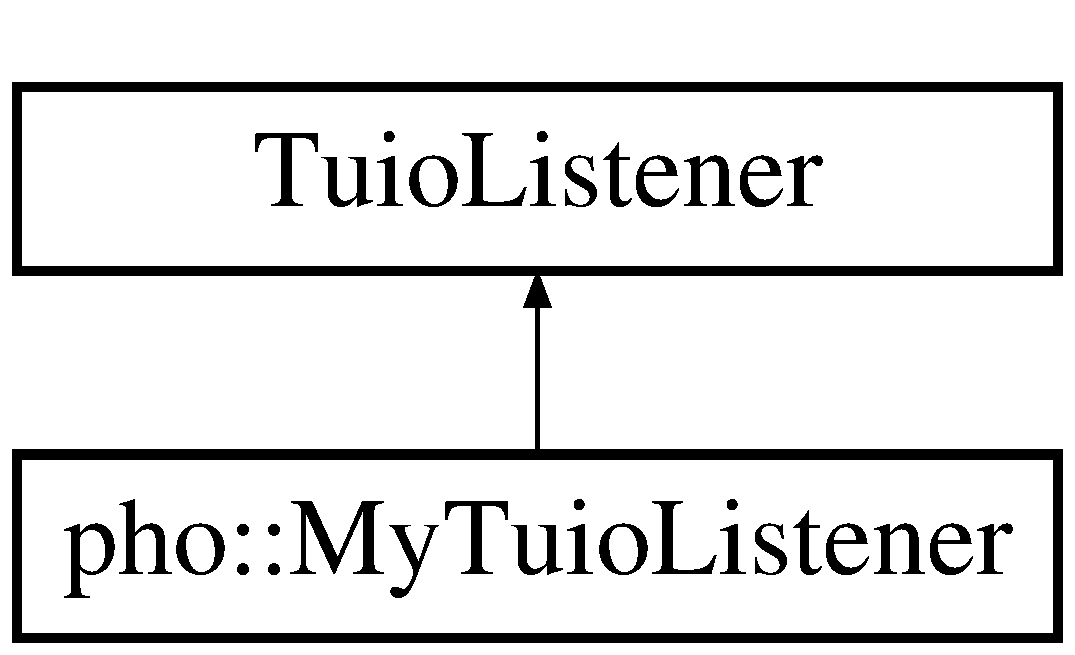
\includegraphics[height=2.000000cm]{classpho_1_1MyTuioListener}
\end{center}
\end{figure}
\subsection*{Public Member Functions}
\begin{DoxyCompactItemize}
\item 
\hypertarget{classpho_1_1MyTuioListener_a723fc12e6a63d9efabe8562a9ae53cb2}{{\bfseries My\-Tuio\-Listener} (int port, \hyperlink{classpho_1_1Engine}{pho\-::\-Engine} $\ast$teh\-Engine)}\label{classpho_1_1MyTuioListener_a723fc12e6a63d9efabe8562a9ae53cb2}

\item 
\hypertarget{classpho_1_1MyTuioListener_a67f3747d7d927ca7e0d8f4a60f8a33ad}{void {\bfseries add\-Tuio\-Object} (Tuio\-Object $\ast$tobj)}\label{classpho_1_1MyTuioListener_a67f3747d7d927ca7e0d8f4a60f8a33ad}

\item 
\hypertarget{classpho_1_1MyTuioListener_ab24eab81f3e7e0f26de1086f0e5e82e4}{void {\bfseries update\-Tuio\-Object} (Tuio\-Object $\ast$tobj)}\label{classpho_1_1MyTuioListener_ab24eab81f3e7e0f26de1086f0e5e82e4}

\item 
\hypertarget{classpho_1_1MyTuioListener_ad97047ec5946ac6d9983baad23e8ab16}{void {\bfseries remove\-Tuio\-Object} (Tuio\-Object $\ast$tobj)}\label{classpho_1_1MyTuioListener_ad97047ec5946ac6d9983baad23e8ab16}

\item 
\hypertarget{classpho_1_1MyTuioListener_a70d7553cb210b29c61ad1a0b7b44c8cf}{void {\bfseries add\-Tuio\-Cursor} (Tuio\-Cursor $\ast$tcur)}\label{classpho_1_1MyTuioListener_a70d7553cb210b29c61ad1a0b7b44c8cf}

\item 
\hypertarget{classpho_1_1MyTuioListener_a255070e3b74c2e40be6a1926e75c354a}{void {\bfseries update\-Tuio\-Cursor} (Tuio\-Cursor $\ast$tcur)}\label{classpho_1_1MyTuioListener_a255070e3b74c2e40be6a1926e75c354a}

\item 
\hypertarget{classpho_1_1MyTuioListener_a03eb721df2ac2869abf5894eb5caf24e}{void {\bfseries remove\-Tuio\-Cursor} (Tuio\-Cursor $\ast$tcur)}\label{classpho_1_1MyTuioListener_a03eb721df2ac2869abf5894eb5caf24e}

\item 
\hypertarget{classpho_1_1MyTuioListener_a40fa32b8f8bee2f45434178bc6e943b1}{void {\bfseries refresh} (Tuio\-Time frame\-Time)}\label{classpho_1_1MyTuioListener_a40fa32b8f8bee2f45434178bc6e943b1}

\end{DoxyCompactItemize}
\subsection*{Public Attributes}
\begin{DoxyCompactItemize}
\item 
\hypertarget{classpho_1_1MyTuioListener_a2068c8b36e67dd5582b0b495c5d477e6}{Tuio\-Client $\ast$ {\bfseries tuio\-Client}}\label{classpho_1_1MyTuioListener_a2068c8b36e67dd5582b0b495c5d477e6}

\end{DoxyCompactItemize}


The documentation for this class was generated from the following files\-:\begin{DoxyCompactItemize}
\item 
my\-Tuio.\-h\item 
my\-Tuio.\-cpp\end{DoxyCompactItemize}

\hypertarget{classudp__server}{\section{udp\-\_\-server Class Reference}
\label{classudp__server}\index{udp\-\_\-server@{udp\-\_\-server}}
}
\subsection*{Public Member Functions}
\begin{DoxyCompactItemize}
\item 
\hypertarget{classudp__server_a02cdf77fb35a70b1ab817805a76d22e7}{{\bfseries udp\-\_\-server} (boost\-::asio\-::io\-\_\-service \&io\-\_\-service, \hyperlink{classpho_1_1EventQueue}{Event\-Queue} $\ast$Queue, boost\-::mutex $\ast$mutex)}\label{classudp__server_a02cdf77fb35a70b1ab817805a76d22e7}

\end{DoxyCompactItemize}


The documentation for this class was generated from the following files\-:\begin{DoxyCompactItemize}
\item 
asio.\-h\item 
asio.\-cpp\end{DoxyCompactItemize}

\hypertarget{classpho_1_1Vector3}{\section{pho\-:\-:Vector3 Class Reference}
\label{classpho_1_1Vector3}\index{pho\-::\-Vector3@{pho\-::\-Vector3}}
}
\subsection*{Public Member Functions}
\begin{DoxyCompactItemize}
\item 
\hypertarget{classpho_1_1Vector3_ac454d0cf76326e6e16a52ac46a62ee8f}{{\bfseries Vector3} (float x, float y, float z)}\label{classpho_1_1Vector3_ac454d0cf76326e6e16a52ac46a62ee8f}

\item 
\hypertarget{classpho_1_1Vector3_a2126f49b2dd9d4d1dc6ec305b12bad04}{{\bfseries Vector3} (const \hyperlink{classpho_1_1Vector3}{Vector3} \&v)}\label{classpho_1_1Vector3_a2126f49b2dd9d4d1dc6ec305b12bad04}

\item 
\hypertarget{classpho_1_1Vector3_a524e426fc1c01190618640d45f8bc730}{float {\bfseries x} () const }\label{classpho_1_1Vector3_a524e426fc1c01190618640d45f8bc730}

\item 
\hypertarget{classpho_1_1Vector3_aaf967c14c11eb003aca9ec9f3de29bd0}{float {\bfseries y} () const }\label{classpho_1_1Vector3_aaf967c14c11eb003aca9ec9f3de29bd0}

\item 
\hypertarget{classpho_1_1Vector3_a9abf1bfb23662e46a953fee3d53474e6}{float {\bfseries z} () const }\label{classpho_1_1Vector3_a9abf1bfb23662e46a953fee3d53474e6}

\item 
\hypertarget{classpho_1_1Vector3_abcd804a1124a748d3b9ab1c5e8c93d40}{float {\bfseries operator\mbox{[}$\,$\mbox{]}} (int i) const }\label{classpho_1_1Vector3_abcd804a1124a748d3b9ab1c5e8c93d40}

\item 
\hypertarget{classpho_1_1Vector3_a297bd1c6a3690cbb62d6351c1d231a23}{float {\bfseries length} () const }\label{classpho_1_1Vector3_a297bd1c6a3690cbb62d6351c1d231a23}

\item 
\hypertarget{classpho_1_1Vector3_a1495858c806e08eef5a82fce916e7da4}{void {\bfseries normalize} ()}\label{classpho_1_1Vector3_a1495858c806e08eef5a82fce916e7da4}

\item 
\hypertarget{classpho_1_1Vector3_a4af94b6665da066c7cdf01551dc8de62}{\hyperlink{classpho_1_1Vector3}{Vector3} {\bfseries operator+} (const \hyperlink{classpho_1_1Vector3}{Vector3} \&op2) const }\label{classpho_1_1Vector3_a4af94b6665da066c7cdf01551dc8de62}

\item 
\hypertarget{classpho_1_1Vector3_a88c862758680cc154d2fcaecaa8f5cdf}{\hyperlink{classpho_1_1Vector3}{Vector3} {\bfseries operator-\/} (const \hyperlink{classpho_1_1Vector3}{Vector3} \&op2) const }\label{classpho_1_1Vector3_a88c862758680cc154d2fcaecaa8f5cdf}

\item 
\hypertarget{classpho_1_1Vector3_a7d8078d09c5da726686595ef4a1c3603}{\hyperlink{classpho_1_1Vector3}{Vector3} {\bfseries operator-\/} () const }\label{classpho_1_1Vector3_a7d8078d09c5da726686595ef4a1c3603}

\item 
\hypertarget{classpho_1_1Vector3_a4c03a93a8f417b62c0624f2197a54431}{\hyperlink{classpho_1_1Vector3}{Vector3} {\bfseries operator$\ast$} (float s) const }\label{classpho_1_1Vector3_a4c03a93a8f417b62c0624f2197a54431}

\item 
\hypertarget{classpho_1_1Vector3_a8b11597934889b6d74dd60b0b50b2240}{void {\bfseries operator$\ast$=} (float s)}\label{classpho_1_1Vector3_a8b11597934889b6d74dd60b0b50b2240}

\item 
\hypertarget{classpho_1_1Vector3_a46f73cd3d1cf2f0c83fb6b52e9d734fa}{\hyperlink{classpho_1_1Vector3}{Vector3} {\bfseries operator/} (float s) const }\label{classpho_1_1Vector3_a46f73cd3d1cf2f0c83fb6b52e9d734fa}

\item 
\hypertarget{classpho_1_1Vector3_a855059e9e56e042a1806de4e219bd8cf}{float {\bfseries operator$\ast$} (const \hyperlink{classpho_1_1Vector3}{Vector3} \&op2) const }\label{classpho_1_1Vector3_a855059e9e56e042a1806de4e219bd8cf}

\item 
\hypertarget{classpho_1_1Vector3_ab4477de79b62cb3c23b50bcdf542acf6}{\hyperlink{classpho_1_1Vector3}{Vector3} {\bfseries operator$^\wedge$} (const \hyperlink{classpho_1_1Vector3}{Vector3} \&op2) const }\label{classpho_1_1Vector3_ab4477de79b62cb3c23b50bcdf542acf6}

\item 
\hypertarget{classpho_1_1Vector3_ae7c2fada3ff78fca4b13ec33245b92e4}{bool {\bfseries operator==} (const \hyperlink{classpho_1_1Vector3}{Vector3} \&op2) const }\label{classpho_1_1Vector3_ae7c2fada3ff78fca4b13ec33245b92e4}

\item 
\hypertarget{classpho_1_1Vector3_ab9a92218aa879dd463ef782044527798}{bool {\bfseries operator!=} (const \hyperlink{classpho_1_1Vector3}{Vector3} \&op2) const }\label{classpho_1_1Vector3_ab9a92218aa879dd463ef782044527798}

\item 
\hypertarget{classpho_1_1Vector3_ac5bb55b238f78040d7668d3d484deaab}{bool {\bfseries operator$<$} (const \hyperlink{classpho_1_1Vector3}{Vector3} \&op2) const }\label{classpho_1_1Vector3_ac5bb55b238f78040d7668d3d484deaab}

\item 
\hypertarget{classpho_1_1Vector3_ac5ef1a635321a3490dddcd74a71807dc}{bool {\bfseries operator$<$=} (const \hyperlink{classpho_1_1Vector3}{Vector3} \&op2) const }\label{classpho_1_1Vector3_ac5ef1a635321a3490dddcd74a71807dc}

\end{DoxyCompactItemize}


The documentation for this class was generated from the following file\-:\begin{DoxyCompactItemize}
\item 
vector3.\-h\end{DoxyCompactItemize}

\hypertarget{classpho_1_1WiiButtonState}{\section{pho\-:\-:Wii\-Button\-State Class Reference}
\label{classpho_1_1WiiButtonState}\index{pho\-::\-Wii\-Button\-State@{pho\-::\-Wii\-Button\-State}}
}
\subsection*{Public Member Functions}
\begin{DoxyCompactItemize}
\item 
\hypertarget{classpho_1_1WiiButtonState_a2f1ec7e94e22616ce408d8e72f8424dd}{void {\bfseries reset} ()}\label{classpho_1_1WiiButtonState_a2f1ec7e94e22616ce408d8e72f8424dd}

\end{DoxyCompactItemize}
\subsection*{Public Attributes}
\begin{DoxyCompactItemize}
\item 
\hypertarget{classpho_1_1WiiButtonState_afd8bddaf031899dd3e6f98ad305599a7}{bool {\bfseries a}}\label{classpho_1_1WiiButtonState_afd8bddaf031899dd3e6f98ad305599a7}

\item 
\hypertarget{classpho_1_1WiiButtonState_a72a01e20f4601c2256483b8af6cc7045}{bool {\bfseries b}}\label{classpho_1_1WiiButtonState_a72a01e20f4601c2256483b8af6cc7045}

\item 
\hypertarget{classpho_1_1WiiButtonState_a3075e54656715000d168184fb2422657}{bool {\bfseries power}}\label{classpho_1_1WiiButtonState_a3075e54656715000d168184fb2422657}

\item 
\hypertarget{classpho_1_1WiiButtonState_a6400af1470deeefbdf369afaf2c83876}{bool {\bfseries plus}}\label{classpho_1_1WiiButtonState_a6400af1470deeefbdf369afaf2c83876}

\item 
\hypertarget{classpho_1_1WiiButtonState_a6c4e6295279a3471ed831ff013dd41e0}{bool {\bfseries minus}}\label{classpho_1_1WiiButtonState_a6c4e6295279a3471ed831ff013dd41e0}

\item 
\hypertarget{classpho_1_1WiiButtonState_ada3420cdc152042a572fefc0e8d5c94b}{bool {\bfseries home}}\label{classpho_1_1WiiButtonState_ada3420cdc152042a572fefc0e8d5c94b}

\item 
\hypertarget{classpho_1_1WiiButtonState_a6db66636181d5489834ac3b16cbcc0b5}{bool {\bfseries one}}\label{classpho_1_1WiiButtonState_a6db66636181d5489834ac3b16cbcc0b5}

\item 
\hypertarget{classpho_1_1WiiButtonState_ab5b313eec50cf41aaf6b821004b5cdd5}{bool {\bfseries two}}\label{classpho_1_1WiiButtonState_ab5b313eec50cf41aaf6b821004b5cdd5}

\item 
\hypertarget{classpho_1_1WiiButtonState_a44e7ec21d363af4c9ced366d74164a4f}{bool {\bfseries down}}\label{classpho_1_1WiiButtonState_a44e7ec21d363af4c9ced366d74164a4f}

\item 
\hypertarget{classpho_1_1WiiButtonState_accdfeb203272d06ddd7d72415980b6d7}{bool {\bfseries up}}\label{classpho_1_1WiiButtonState_accdfeb203272d06ddd7d72415980b6d7}

\item 
\hypertarget{classpho_1_1WiiButtonState_a8b9824d50a2b20a926644f4e169d86df}{bool {\bfseries left}}\label{classpho_1_1WiiButtonState_a8b9824d50a2b20a926644f4e169d86df}

\item 
\hypertarget{classpho_1_1WiiButtonState_a5079d6e145b61c14c8d3a9b639de940f}{bool {\bfseries right}}\label{classpho_1_1WiiButtonState_a5079d6e145b61c14c8d3a9b639de940f}

\end{DoxyCompactItemize}


The documentation for this class was generated from the following files\-:\begin{DoxyCompactItemize}
\item 
util.\-h\item 
util.\-cpp\end{DoxyCompactItemize}

\addcontentsline{toc}{part}{Index}
\printindex
\end{document}
